%%%%%%%%%%%%%%%%%%%%%%%%%%%%%%%%%%%%%%%%%%%%%%%%%%%%%%%%%%%%%%%%%%%%%%%%
%    INSTITUTE OF PHYSICS PUBLISHING                                   %
%                                                                      %
%   `Preparing an article for publication in an Institute of Physics   %
%    Publishing journal using LaTeX'                                   %
%                                                                      %
%    LaTeX source code `ioplau2e.tex' used to generate `author         %
%    guidelines', the documentation explaining and demonstrating use   %
%    of the Institute of Physics Publishing LaTeX preprint files       %
%    `iopart.cls, iopart12.clo and iopart10.clo'.                      %
%                                                                      %
%    `ioplau2e.tex' itself uses LaTeX with `iopart.cls'                %
%                                                                      %
%%%%%%%%%%%%%%%%%%%%%%%%%%%%%%%%%%
%
%
% First we have a character check
%
% ! exclamation mark    " double quote  
% # hash                ` opening quote (grave)
% & ampersand           ' closing quote (acute)
% $ dollar              % percent       
% ( open parenthesis    ) close paren.  
% - hyphen              = equals sign
% | vertical bar        ~ tilde         
% @ at sign             _ underscore
% { open curly brace    } close curly   
% [ open square         ] close square bracket
% + plus sign           ; semi-colon    
% * asterisk            : colon
% < open angle bracket  > close angle   
% , comma               . full stop
% ? question mark       / forward slash 
% \ backslash           ^ circumflex
%
% ABCDEFGHIJKLMNOPQRSTUVWXYZ 
% abcdefghijklmnopqrstuvwxyz 
% 1234567890
%
%%%%%%%%%%%%%%%%%%%%%%%%%%%%%%%%%%%%%%%%%%%%%%%%%%%%%%%%%%%%%%%%%%%
%
\documentclass[12pt]{iopart}
\usepackage{graphicx}
\usepackage{subcaption}

\usepackage{amsfonts}
\expandafter\let\csname equation*\endcsname\relax

\expandafter\let\csname endequation*\endcsname\relax

\usepackage{amsmath}
\usepackage{listings}

\usepackage[most]{tcolorbox}

\definecolor{bg}{RGB}{255,249,227}
\definecolor{light_orange}{RGB}{255,193,134}

\newtcolorbox{optional}[1][]{%
enhanced jigsaw,
%oversize,
colback=bg,
boxrule=0pt,
overlay unbroken and first ={%
\draw[line width=0.2pt,double=bg,draw=bg!70!black,
    double distance=1pt,] (frame.north west) -- (frame.north east);
\draw[line width=0.2pt,double=bg,draw=bg!70!black,
    double distance=1pt,] (frame.south west) -- (frame.south east);},
breakable,
arc=0pt,outer arc=0pt,
#1}%

\newtcolorbox{tldr}[1][]{%
enhanced jigsaw,
%oversize,
colback=light_orange,
boxrule=0pt,
overlay unbroken and first ={%
\draw[line width=0.2pt,double=bg,draw=bg!70!black,
    double distance=1pt,] (frame.north west) -- (frame.north east);
\draw[line width=0.2pt,double=bg,draw=bg!70!black,
    double distance=1pt,] (frame.south west) -- (frame.south east);},
breakable,
arc=0pt,outer arc=0pt,
#1}%


\definecolor{codegreen}{rgb}{0,0.6,0}
\definecolor{codegray}{rgb}{0.5,0.5,0.5}
\definecolor{codepurple}{rgb}{0.58,0,0.82}
\definecolor{backcolour}{rgb}{0.95,0.95,0.92}

\lstdefinestyle{mystyle}{
    backgroundcolor=\color{backcolour},   
    commentstyle=\color{codegreen},
    keywordstyle=\color{magenta},
    numberstyle=\tiny\color{codegray},
    stringstyle=\color{codepurple},
    % basicstyle=\ttfamily\footnotesize,
    basicstyle=\ttfamily,
    breakatwhitespace=false,         
    breaklines=true,                 
    captionpos=b,                    
    keepspaces=true,                 
    numbers=left,                    
    numbersep=5pt,                  
    showspaces=false,                
    showstringspaces=false,
    showtabs=false,                  
    tabsize=2
}
\lstMakeShortInline[columns=fixed]!
\lstset{style=mystyle}


%Uncomment next line if AMS fonts required
%\usepackage{iopams}  
\begin{document}

\title{A practical guide to Digital Micro-mirror Devices (DMDs) for wavefront shaping}

\author{Sébastien M. Popoff}
\address{Institut Langevin, ESPCI Paris, PSL University, CNRS, France}
\ead{sebastien.popoff@espci.psl.eu}

\author{Rodrigo Gutiérrez-Cuevas}
\address{Institut Langevin, ESPCI Paris, PSL University, CNRS, France}
\ead{rodrigo.gutierrez-cuevas@espci.psl.eu>}

\author{Yaron Bromberg}
\address{Racah Institute of Physics, The Hebrew University of Jerusalem, Israel}

\author{Maxime W. Matthès}
\address{Institut Langevin, ESPCI Paris, PSL University, CNRS, France}

% \address{IOP Publishing, Temple Circus, Temple Way, Bristol BS1 6HG, UK}
\vspace{10pt}
\begin{indented}
\item[]September 2023
\end{indented}

\begin{abstract}
Abstract
\end{abstract}

%
% Uncomment for keywords
%\vspace{2pc}
%\noindent{\it Keywords}: XXXXXX, YYYYYYYY, ZZZZZZZZZ
%
% Uncomment for Submitted to journal title message
%\submitto{\JPA}
%
% Uncomment if a separate title page is required
%\maketitle
% 
% For two-column output uncomment the next line and choose [10pt] rather than [12pt] in the \documentclass declaration
%\ioptwocol
%

\section{Introduction}

Since the advent of adaptive optics, various technologies have been employed 
to modulate the amplitude and/or phase of light. 
Early adaptive optics devices, utilized in fields like microscopy and astronomy, 
offer rapid modulation capable of compensating for the aberrations of optical systems 
in real-time. 
However, these devices are constrained by a limited number of actuators, 
restricting their utility in complex media where a large number of degrees of freedom is essential. 
Liquid Crystal Spatial Light Modulators (LC-SLMs), 
which allow for the control of light phase across typically more than a million pixels, 
have emerged as powerful tools for wavefront shaping in complex media 
since the seminal work of A. Most and I. Vellekoop in the mid-2000s~\cite{Vellekoop2007focusing}. 
Nonetheless, LC-SLMs are hampered by their slow response time, 
permitting only a modulation speed ranging from a few Hz to about 100 Hz. 
Digital Micromirror Devices (DMDs) have emerged as a technology bridging the gap 
between these two types of systems; 
they offer a large number of pixels (similar to LC-SLMs) and fast modulation speeds (typically up to several tens of kHz). 
However, DMDs are restricted to binary amplitude modulation and are not optimized for coherent light applications. 
Utilizing DMDs for coherent control of light in complex media is therefore non-trivial 
and necessitates specific adaptations for efficient use. 
This tutorial aims to provide a comprehensive guide 
for selecting and employing DMDs in wavefront shaping applications within complex media.\\



To comprehend both the capabilities and limitations
of DMD technology for coherent wavefront shaping,
it is crucial to understand the device's operating principles
and its original design intentions.
Investigated and developed by Texas Instruments since the late 1970s,
DMDs gained prominence in the 1990s for video projection applications
under the commercial name of Digital Light Processing (DLP)~\cite{Dudley2003emerging}.
The technology enables high-resolution, high-speed, and high-contrast-ratio modulation of light.\\
DMDs operate by toggling the state of small mirrors between two distinct angles, denoted as $\pm \theta_\text{DMD}$.
The device is originally engineered for amplitude modulation in video projection applications.
In this configuration, one mirror angle directs light into the projection lens,
while the alternate angle results in the light path being blocked (see Fig~\ref{fig:combined_pixel}).
Given that projectors utilize incoherent light and that the DMD plane is optically conjugated with the projection screen,
aberrations within the DMD plane are generally not problematic.
Similarly, phase fluctuations induced by temperature variations, 
as well as minor vibrations from the cooling hardware, are inconsequential in this context.
The DMD is designed to produce binary on/off modulation,
which is then leveraged to generate grayscale images via pulse-width modulation.
Color modulation is accomplished through the use of a color wheel in conjunction with a bright white light source.\\

Third-party companies have developped kits for research applications,
providing a DMD with a control board and a software interface. 
In particular, Vialux devices~\cite{}, provides a FPGA board that enable high speed modulation 
by allowing frames to be stored in the device memory. 
However, sandard Texas Instrument video projector evaluation modules can be converted into a wavefront shaping device~\cite{Cox2021converting}, 
albeit with a lower modulation speed.
Such systems can then be converted into phase or complex field modulators. 
It typically relies on encoding the optical phase into 
the spatial displacement of binaray spatial fringes displayed on the DMD 
and then filtering the high spatial frequencies in the Fourier plane~\cite{Lee1979binary}.
It allows multiple level complex modulation at the expense of a reduced spatial resolution.
The implementation and the performance of such a system are studied in a separate tutorial~\cite{RODRIGO} 
and will not be detailed here.
In the rest of the paper, we will assume that the DMD is used for complex modulation using such an approach.
While the present tutorial is not specific to any particular device, 
the software section will focus on the Vialux control board.
In a first part....\\


\begin{figure}
\centering
\begin{subfigure}{0.49\textwidth}
\centering
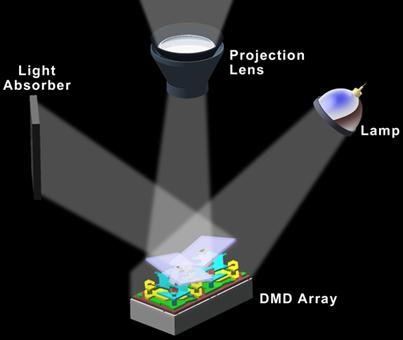
\includegraphics[width = \textwidth]{images/pixel_1.jpg}
\label{fig:pix_left}
\end{subfigure}
\begin{subfigure}{0.49\textwidth}
\centering
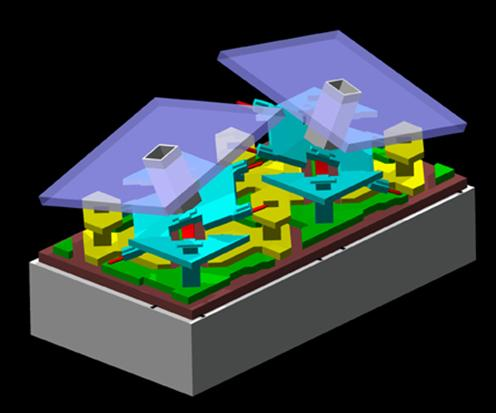
\includegraphics[width = \textwidth]{images/pixel_2.jpg}
\label{fig:pix_right}
\end{subfigure}
\caption{
\textbf{Principle of operation of a DMD in a digital projector.}
Left, incident light can be reflected towards the projection lens (state {\em on}), 
or onto a beam dump (state {\em off}).
Right, zoom on the pixels. 
Image adapted from \cite{JacksonDMD}.
}
\label{fig:combined_pixel}
\end{figure}




% \cite{JacksonDMD}



\section{Choosing the right DMD: Diffraction effects}

\subsection{1D model}

One important difference between liquid crystal modulators and DMDs 
concerns the geometry of the pixel surface. 
This leads to diffraction effects that can be detrimental 
to the modulation and efficiency of the system.
It strongly depends on the wavelength of the illumination, 
the pixel pitch, and the incident and outgoing angles. 
Thus, in addition to choosing an appropriate anti-reflection coating, 
it is important to check that the pixel pitch is well-suited for the configuration used.
Texas Instruments chips come with different possible pixel pitch $d$ 
ranging roughly from $5$ to $\sim25$\textmu m\cite{TI}.\\


Let's consider a 1D system,
as illustrated in Fig.~\ref{fig:grating_geom},  
% For the sake of simplicity and 
to qualitatively understand the problem.
% we place ourselves in the small angle approximation. 
This corresponds to incident and outgoing angles close to normal to the modulator surface 
and to a small tilt angle of the mirror. 
% We will give latter the final formulas in the 2D case.
We first assume that all the pixels are in the same state 
and are illuminated by a plane wave from the far field.
A pixelated modulator then acts exactly as a grating, 
with a period $d$ equal to the pixel pitch.
Modulators have a filling fraction limited by the hardware, 
typically around 90\%.
This corresponds to having an effective size of active pixels of $d' < d$.

In general, a grating leads to the observation of diffraction orders  
with varying intensities 
and angles $\theta_p$ given by the grating equation
$\text{sin}(\theta_p) = p\lambda/d = p \text{sin}(\theta_D)$,
where $\lambda$ is the wavelength of the light 
and $\theta_D$ the angle of the first order of diffraction.
The intensity of the diffraction orders depends on the size and the response of one pixel.
We see that we can decouple the effect of the periodicity of the grating, 
that acts on the angles of the orders of diffraction, 
and the response of one pixel, 
that acts on the envelope of the angular response.

\begin{figure}
  \centering
  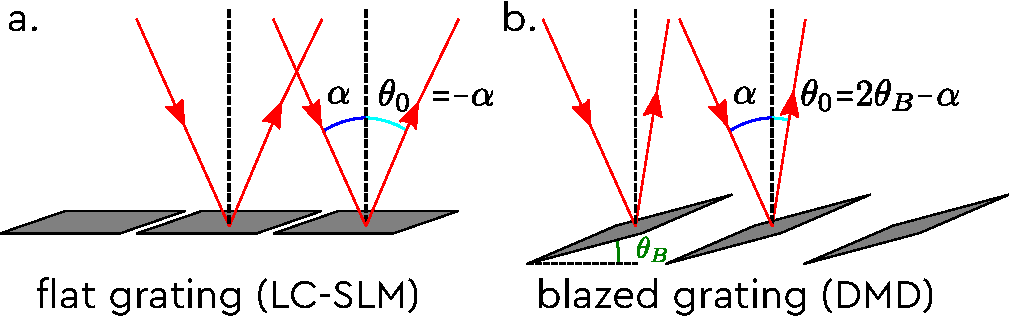
\includegraphics[width = \textwidth]{images/grating_geom.pdf}
  \label{fig:flat_grating}

  \caption{
  \textbf{1D grating geometry.}
 ...
  }
  \label{fig:grating_geom}
  \end{figure}


For a normal incidence 
in the case of a LC-SLM, the response of one pixel is 
assumed constant over the pixel size. 
For a blazed grating, we also have a linear phase slope on each pixel due to the tilt $\theta_B$ of the pixels.
For an an arbitrary incidence angle $\alpha$, we also have a global phase slope 
that has the effect of trivially shifting the angular diffraction by an angle $\alpha$.\\

In essence, the incident angle $\alpha$ has the effect to shift the whole angular diffraction pattern 
with respect to the normal incidence case, 
while the blazed angle $\theta_B$, the tilt angle of the mirror in the DMD, 
has the effect to shift only the envelope by $2\theta_B$.
When the filling fraction is close to 100\%, 
i.e. $d\approx d'$,
the enveloppe for a flat grating is maximal 
at $\theta_0=-\alpha$ corresponding to the angle of the zero-th order,
and close to zero for the other orders.
We then observe a single diffraction order, 
which corresponds to the ideal case.
Adding a blazed angle $\theta_B$ leads to a shift of the envelope, 
the position of the maximum 
$\theta_0=2\theta_B-\alpha$ 
may not correspond anymore to a diffraction order.\\

\begin{optional}
  If we neglect the finite size of the device and illumination 
  and place ourselves in the small angle approximation, 
  we can write the field reflected off the device 
  for a plane wave illumination
  in the two systems as: 

  \begin{equation}
  \begin{aligned}
    R_\text{flat}(x) &\propto \left[\Pi\left(x/d'\right) \otimes_x \sum_k \delta(x-k d)\right]e^{-j\frac{2\pi}{\lambda}\text{sin}(\alpha) x} \\
    R_\text{blazed}(x) &\propto 
        \underbrace{
          \left(
            \underbrace{\Pi\left(x/d'\right)}_\text{pixel size}
              \times 
              \underbrace{e^{j\frac{2\pi}{\lambda}2\text{sin}(\theta_B-\alpha) x}}_{\substack{\text{blazed angle} \\ \text{+ angle of incidence}}}
              %\text{blazed angle + angle of incidence}
          \right) 
        }_\text{pixel response}
        \otimes_x 
        \left[
        \underbrace{\sum_k \delta(x-k d) }_\text{periodicitiy}
        .
        \underbrace{
        e^{-j\frac{2\pi}{\lambda}\text{sin}(\alpha) kd}
      }_\text{angle of incidence}
      \right]
      \, ,
  \end{aligned}
  \label{eq:grating_response}
  \end{equation}

  with $\Pi(x)$ the rectangular function,
  representing the finite size of the pixel, 
  defined as:

  \begin{equation}
    \Pi(x) = 
    \begin{cases}
    1, & \text{if } -\frac{1}{2} < x < \frac{1}{2}, \\
    0, & \text{otherwise}.
    \end{cases}
    \end{equation}

  The intensity as a function of the angle in the far-field 
  is given, up to a homotetic transformation, 
  by the absolute value squared of 
  Fourier transform of Eq.~\ref{eq:grating_response}
  and reads: 


  \begin{equation}
    \begin{aligned}
      I_\text{flat}(\theta) \propto 
        \sum_p \delta(\text{sin}(\theta)+\text{sin}(\alpha)-p\,\theta_D) 
          \times 
        \text{sinc}^2\left( (\text{sin}(\theta)+\text{sin}(\alpha)) \frac{\lambda}{d'}\right)\\
        I_\text{blazed}(\theta) \propto 
        \underbrace{
          \sum_p \delta(\text{sin}(\theta)+\text{sin}(\alpha)-p\,\theta_D) 
        }_\text{orders of diffraction}
        \times 
        \underbrace{
          \text{sinc}^2\left( (\text{sin}(\theta)+\text{sin}(2\theta_B-\alpha)) \frac{\lambda}{d'}\right)
         }_\text{envelope} \, .
    \end{aligned}
  \end{equation}

\end{optional}
A more accurate computation of the far field can be found  in ~\cite{Wang2023diffraction}.
We observe that the envelope (right hand term) is maximal for $\text{sin}(\theta_{max}) = \text{sin}(\alpha-2\theta_B)$ 
while the effect of the periodicity (left hand term) is maximal for $\text{sin}(\theta_p)+ \text{sin}(\alpha) = p \lambda/d$. 
with $p$ an integer value.
We represent in Fig.~\ref{fig:gratings} the angular response of a flat grating and a blazed grating 
for a 1D filling fraction of 95\% (correponding to a 2D filling fraction of $\approx 90$\%).
For a flat grating, only the zero-th order has a significant and comparable intensity. 
For a blazed grating, in this example close to the worst case scenario, 
two diffraction orders have a significant intensity, 
and other orders also have a non-negligible contributions. 
% This implies that by selecting one order, we can loose more that 50\% of the light. 
% In a 2D system, we can then loose more that 75\% of the light.\\ 
The ideal case, i.e. when the maximum of the envelope corresponds to a diffraction order,
leading a single diffraction order containing most of the energy,
is obtained when the blazed grating equation is satistied~\cite{Casini2014on}:

\begin{equation}
  \text{sin}(2\theta_B-\alpha) + \text{sin}(\alpha) 
    = 2 \,\text{sin}(\theta_B)  \,\text{sin}(\theta_B-\alpha) 
    = p\frac{\lambda}{d} \, .
  \label{eq:blazed_eq}
\end{equation}

% Let's intereprete this qualitatively.
% For flat grating
% the incidence angle $\alpha$ 


\begin{figure}
  \centering
  \begin{subfigure}{0.49\textwidth}
  \centering
  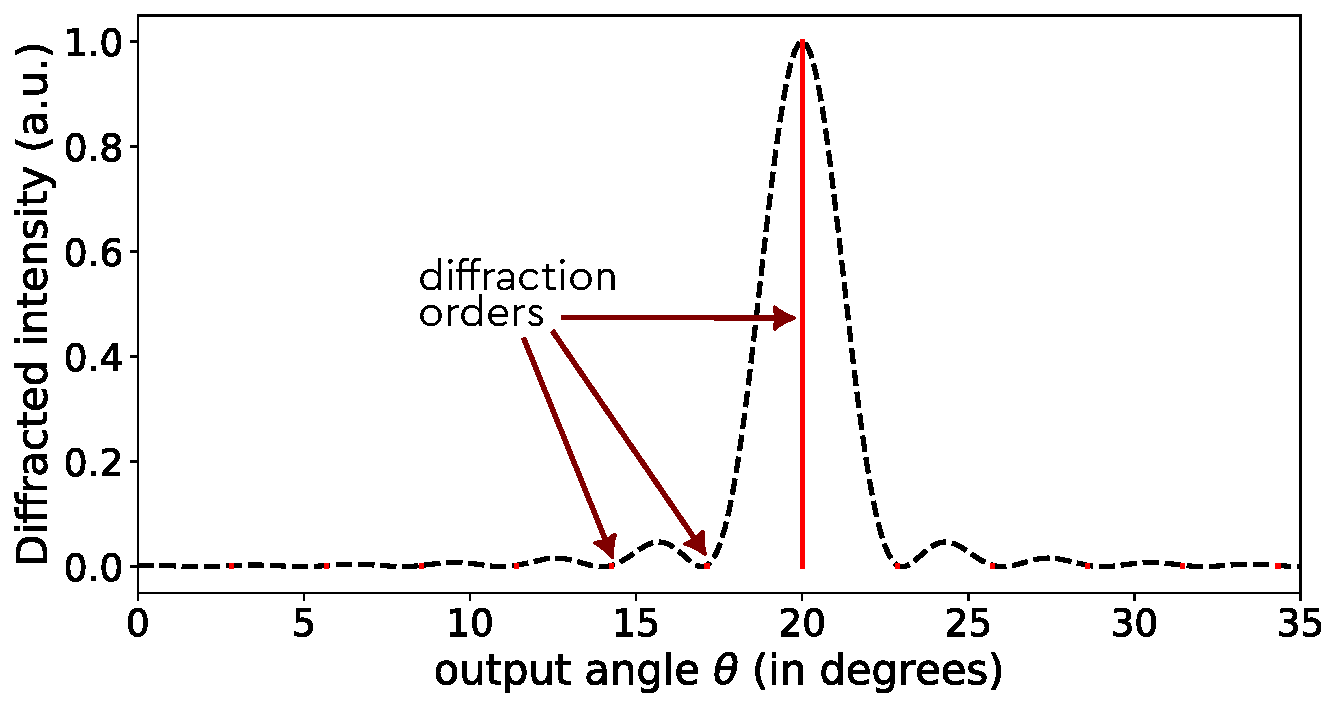
\includegraphics[width = \textwidth]{images/gratings_flat.pdf}
  \label{fig:flat_grating}
  \end{subfigure}
  \begin{subfigure}{0.49\textwidth}
  \centering
  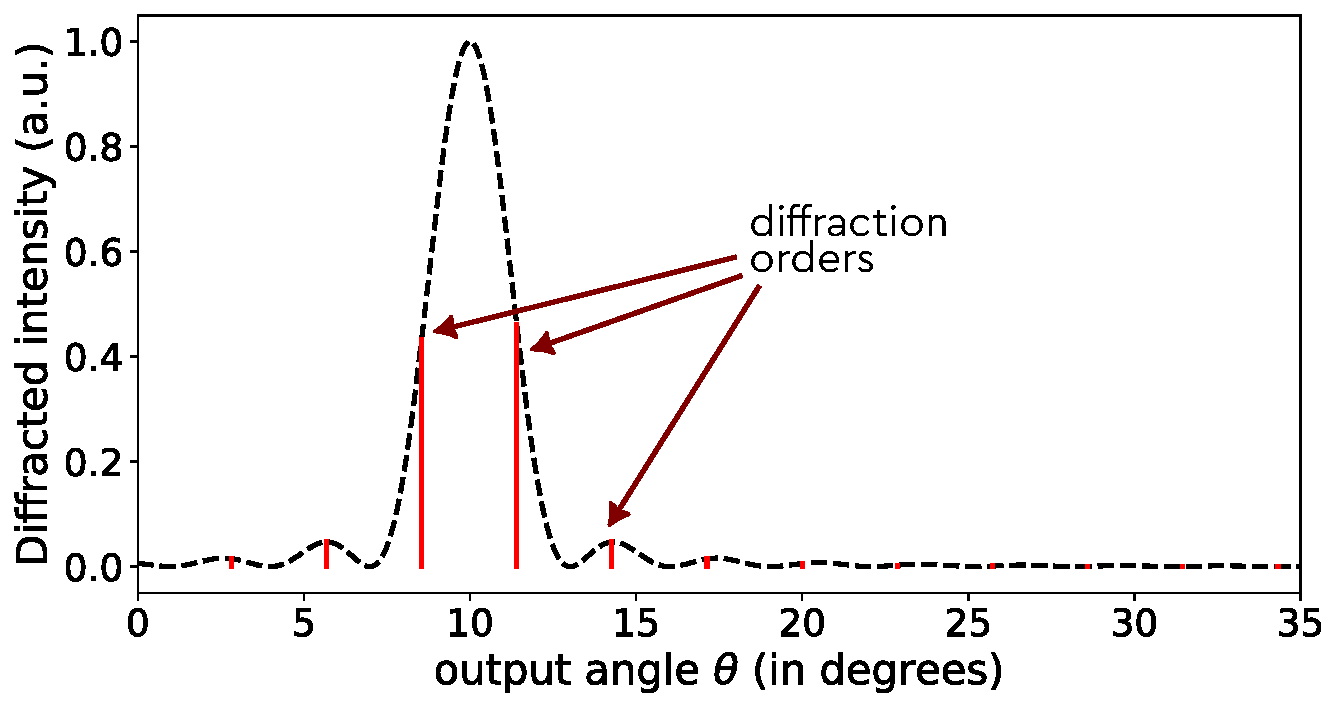
\includegraphics[width = \textwidth]{images/gratings_blazed.pdf}
  \label{fig:blazed_right}
  \end{subfigure}
  \caption{
  \textbf{Flat grating vs blazed grating.}
 ...
  }
  \label{fig:gratings}
  \end{figure}

% \begin{equation}
%     a = 
%   \left\{
%     \begin{aligned}
%         a\\b
% %         x + y   &= 7 \\
% %         5x - 2y &= -7
%     \end{aligned}
%   \right\}
% \end{equation}

% \begin{equation}
%   R_\text{flat}(x) \propto \Pi\left(x/d'\right) \otimes_x \sum_k \delta(x-k d) 
% \end{equation}

% small angle approximation
% \begin{equation}
%   R_\text{blazed}(x) \propto \left[\Pi\left(x/d'\right) \times e^{j\frac{2\pi}{\lambda}\theta_B}\right]\otimes_x \sum_k \delta(x-k d) 
% \end{equation}

\subsection{2D case}

To analyze more precisely the effect of diffraction in a DMD, 
we need to consider the 2D surface of the modulator.
Let's define a cartesian coordinate system in the plane of the DMD
with axis $x$ and $y$ aligned with the pixel sides 
(see Fig.~\ref{fig:2d_geom}a.). 
Pixels are repeated along those directions. 
A technical difficulty is that the axis of rotation of the pixels 
is the diagonal of the pixels, 
hence rotated by 45 degrees with respect to the $x$ and $y$. 
For the alignment and the maniputlation of the optical setup
it is more convenient to work in incident and outgoing beams 
with optical axis contained in an horizontal plane. 
A simple and common solution consists in roatating the chip by 45 degrees
with respect to the horizontal plane 
such that the axis of rotation of the pixels is vertical.  
This configuration is illustrated in Fig.~\ref{fig:2d_geom}.


\begin{figure}
  \centering
  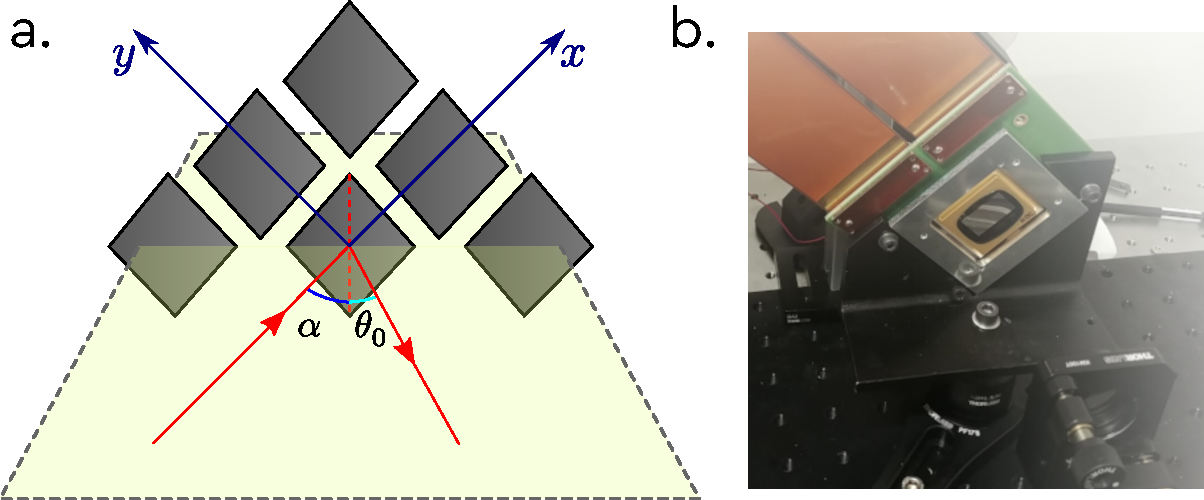
\includegraphics[width = 0.8\textwidth]{images/dmd_45.pdf}
  \caption{
  \textbf{2D grating geometry.}
 ...
  }
  \label{fig:2d_geom}
\end{figure}

The 2D array can be seen as 2 orthogonal 1D gratings in the $x$ and $y$ directions.
The incident angle $\alpha'$. 
Because of the 45 degrees angle between 
axis of rotation of the mirrors and axis, 
both 1D gratings have the same properties. 
A more complete computation of the 2D system can be found in~\cite{Scholes2019structured}.
To apply Eq.~\ref{eq:blazed_eq}, 
we first need to project the 
the different angles of the problem in the incident planes 
of the two 1D gratings.
It gives 
$\alpha = \text{arctan}\left(\text{tan}(\alpha')/\sqrt{2}\right)$, 
$\beta = \text{arctan}\left(\text{tan}(\beta')/\sqrt{2}\right)$, 
and $\theta_B = \text{arctan}\left(\text{tan}(\theta_\text{DMD})/\sqrt{2}\right)$, 
$theta_\text{DMD}$ being the actual rotation angle of the mirrors with respect to the diagonal of the pixels.
We can quantify how close we are to the ideal case, 
i.e. when satifying the blazed equation~\ref{eq:blazed_eq}, 
by defining a {\em blazed number} $\mu$ as~\cite{WFSnet_diffraction}:

\begin{equation}
  \mu =  
  \left|
    \lfloor 2 \frac{d}{\lambda} 
      \left[
        \text{sin}(\alpha)  +\text{sin}(\beta)
      \right] 
    \rfloor
    \mod{2} -1 
  \right| \, ,
\end{equation}

with $\lfloor . \rfloor$ representing the integer part, 
and $\mod{2}$ the modulo 2 operation.
$\mu$ is maximal when the blazing equation is satisfield, 
i.e. when one order of diffraction contains most of the energy, 
and minimal when we are in the worst case scenario, 
i.e. when four orders of diffraction have a significant and equal intensity.\\

To illustrate the effect, we simulate a DMD in Python 
(see tutorial and code in~\cite{WFSnet_diffraction})
with a two pixel pitches of 
$d=7.6$\textmu m and $d=10.8$\textmu m,
for a coherent excitation at $\lambda=633$nm. 
We show in Fig.~\ref{fig:mu76} the blazed number $\mu$
as a function of the incident angle $\alpha'$ 
as well as the far field diffraction pattern for different two incident angles.
While one can change the efficiency of diffraction by tuning 
the incindent angle, its effect is somewhat limited 
withing a reasonable angular range compatible with experimental constraints 
(i.e. for angles far from $\pm 90^\circ$).
Far field pattern are centered around the maximum of the envelope 
$\theta_\text{max} = 2\theta_B - \alpha$ 
(marked by a yellow cross).
We see that for small values of $\alpha$, 
the pixel pitch of $d=10.8$\textmu m leads to a blazed number $\mu$ 
close $1$. 
It corresponds in the far field to having one bright order of diffraction  
close to the maximum of the envelope.

\begin{figure}
  \centering
  \begin{subfigure}{0.49\textwidth}
  \centering
  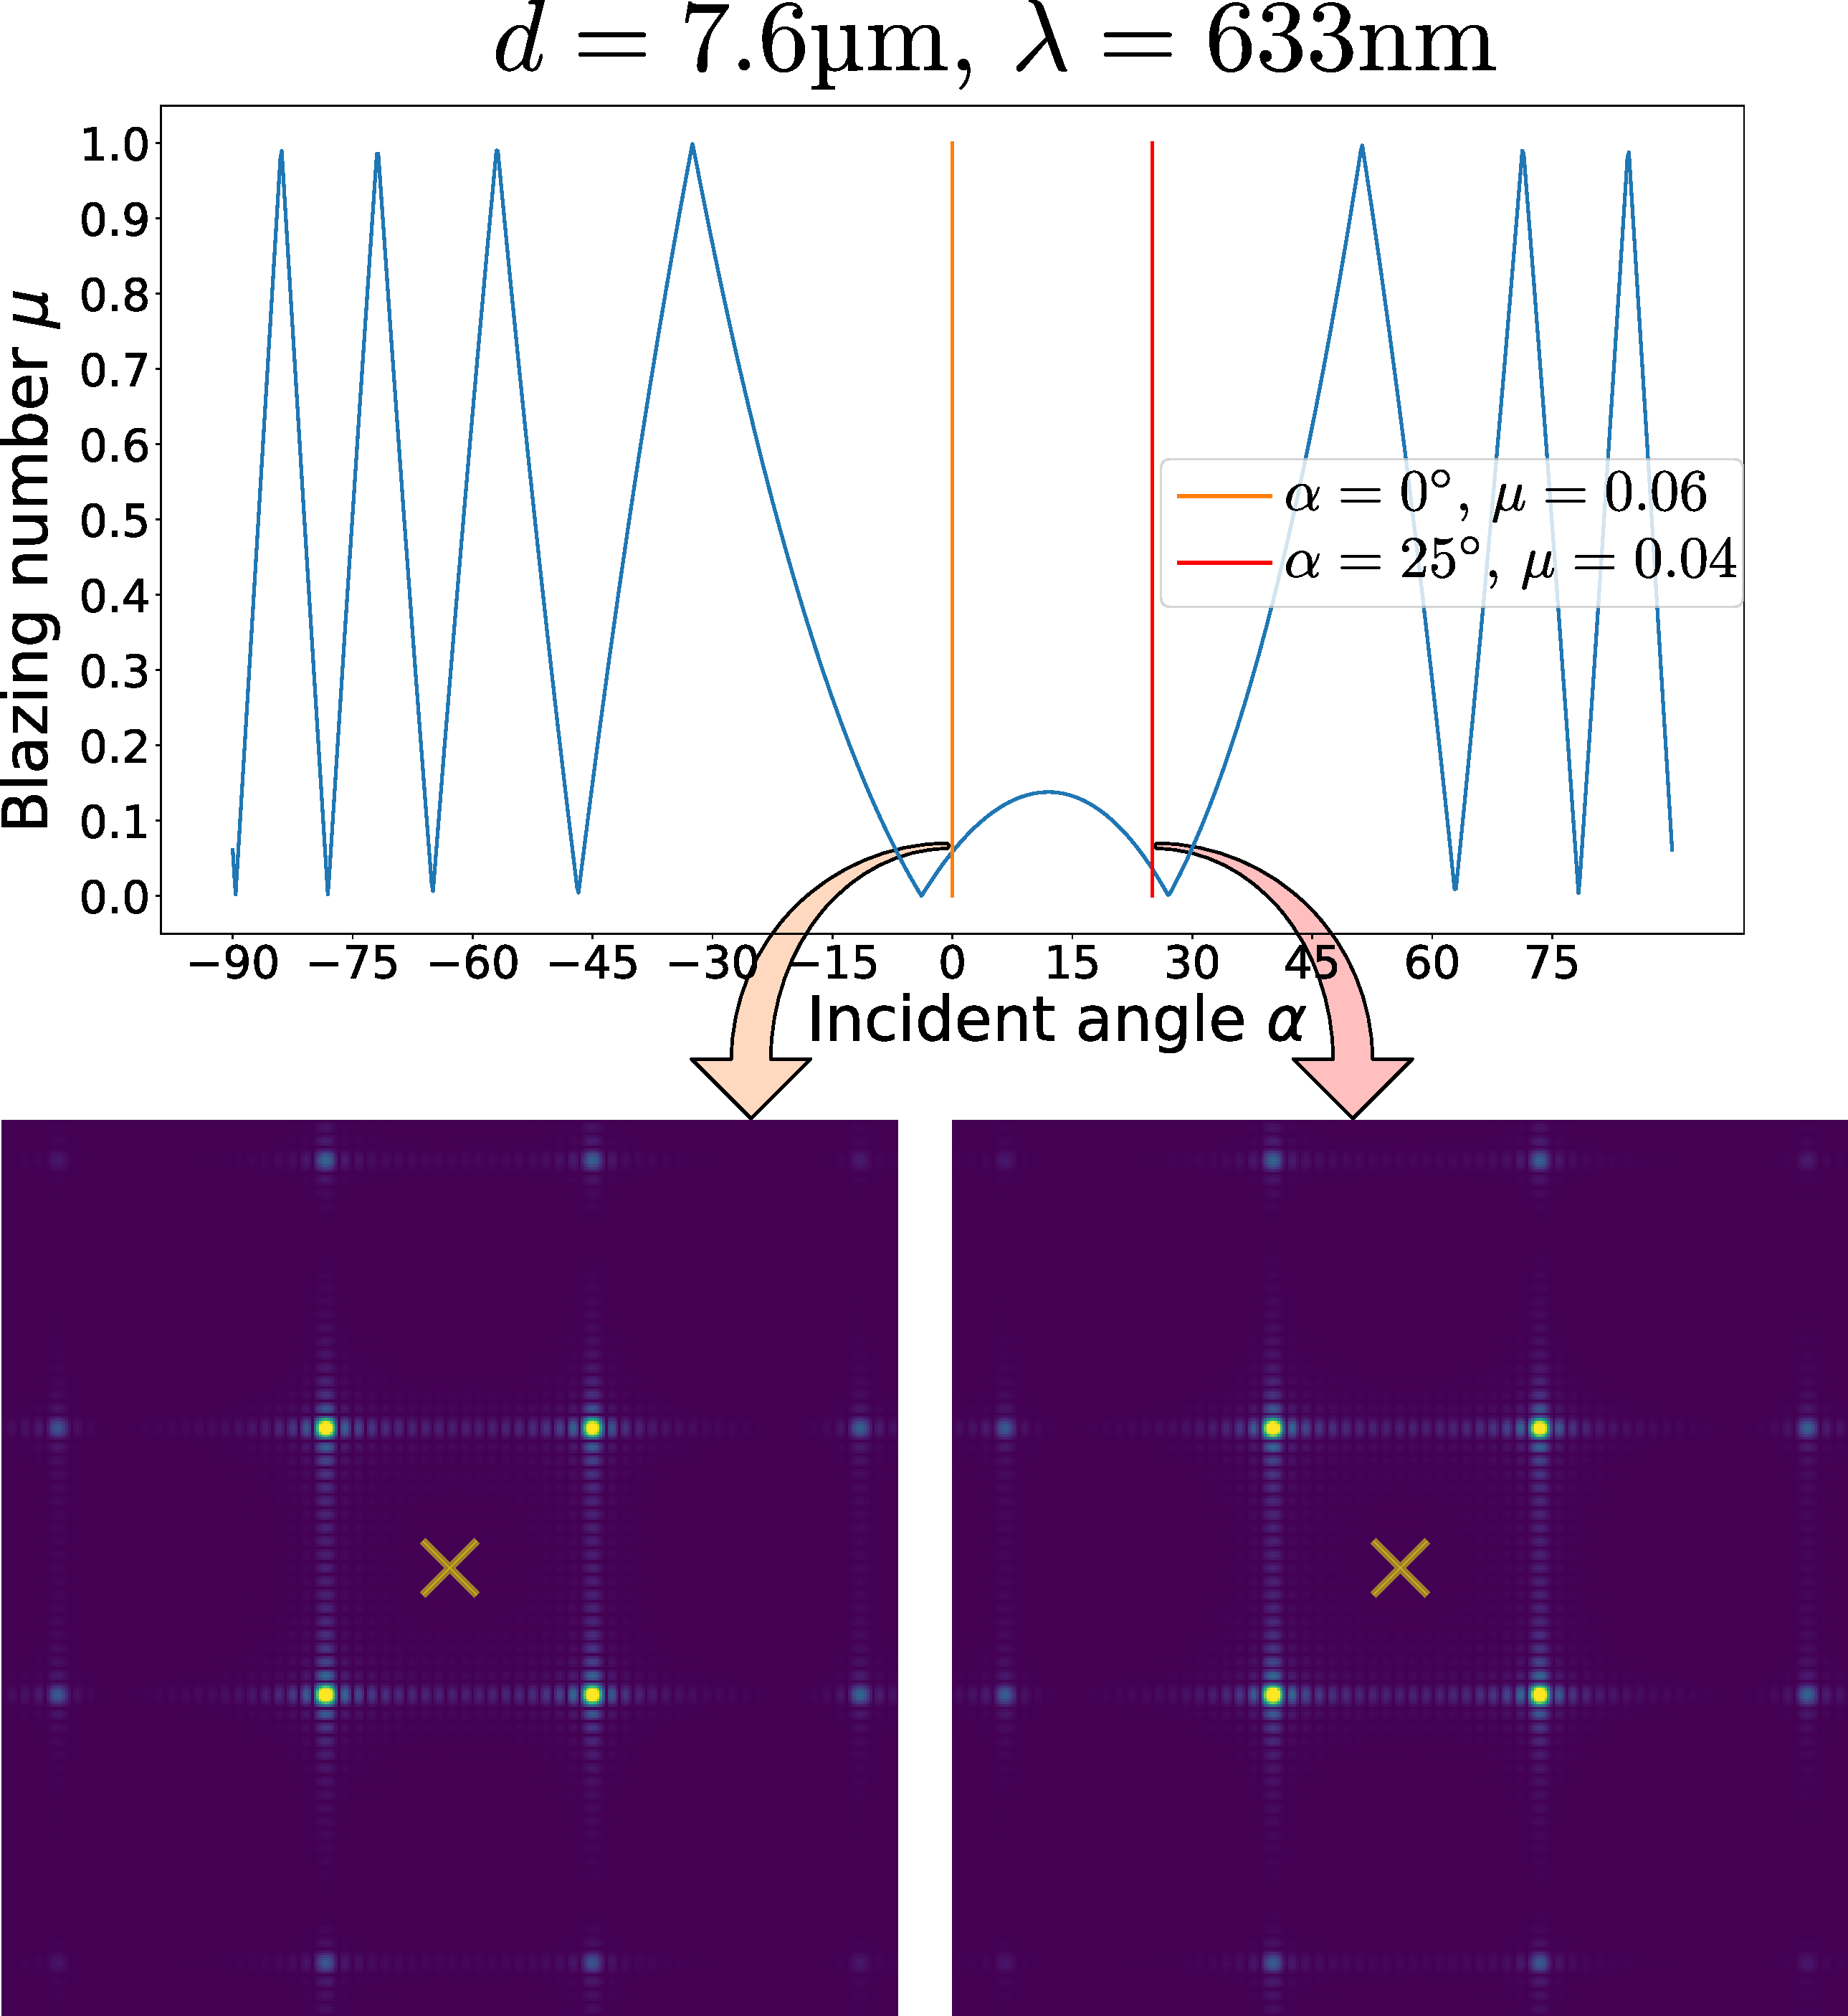
\includegraphics[width = \textwidth]{images/mu_76.pdf}
  \end{subfigure}
  \begin{subfigure}{0.49\textwidth}
  \centering
  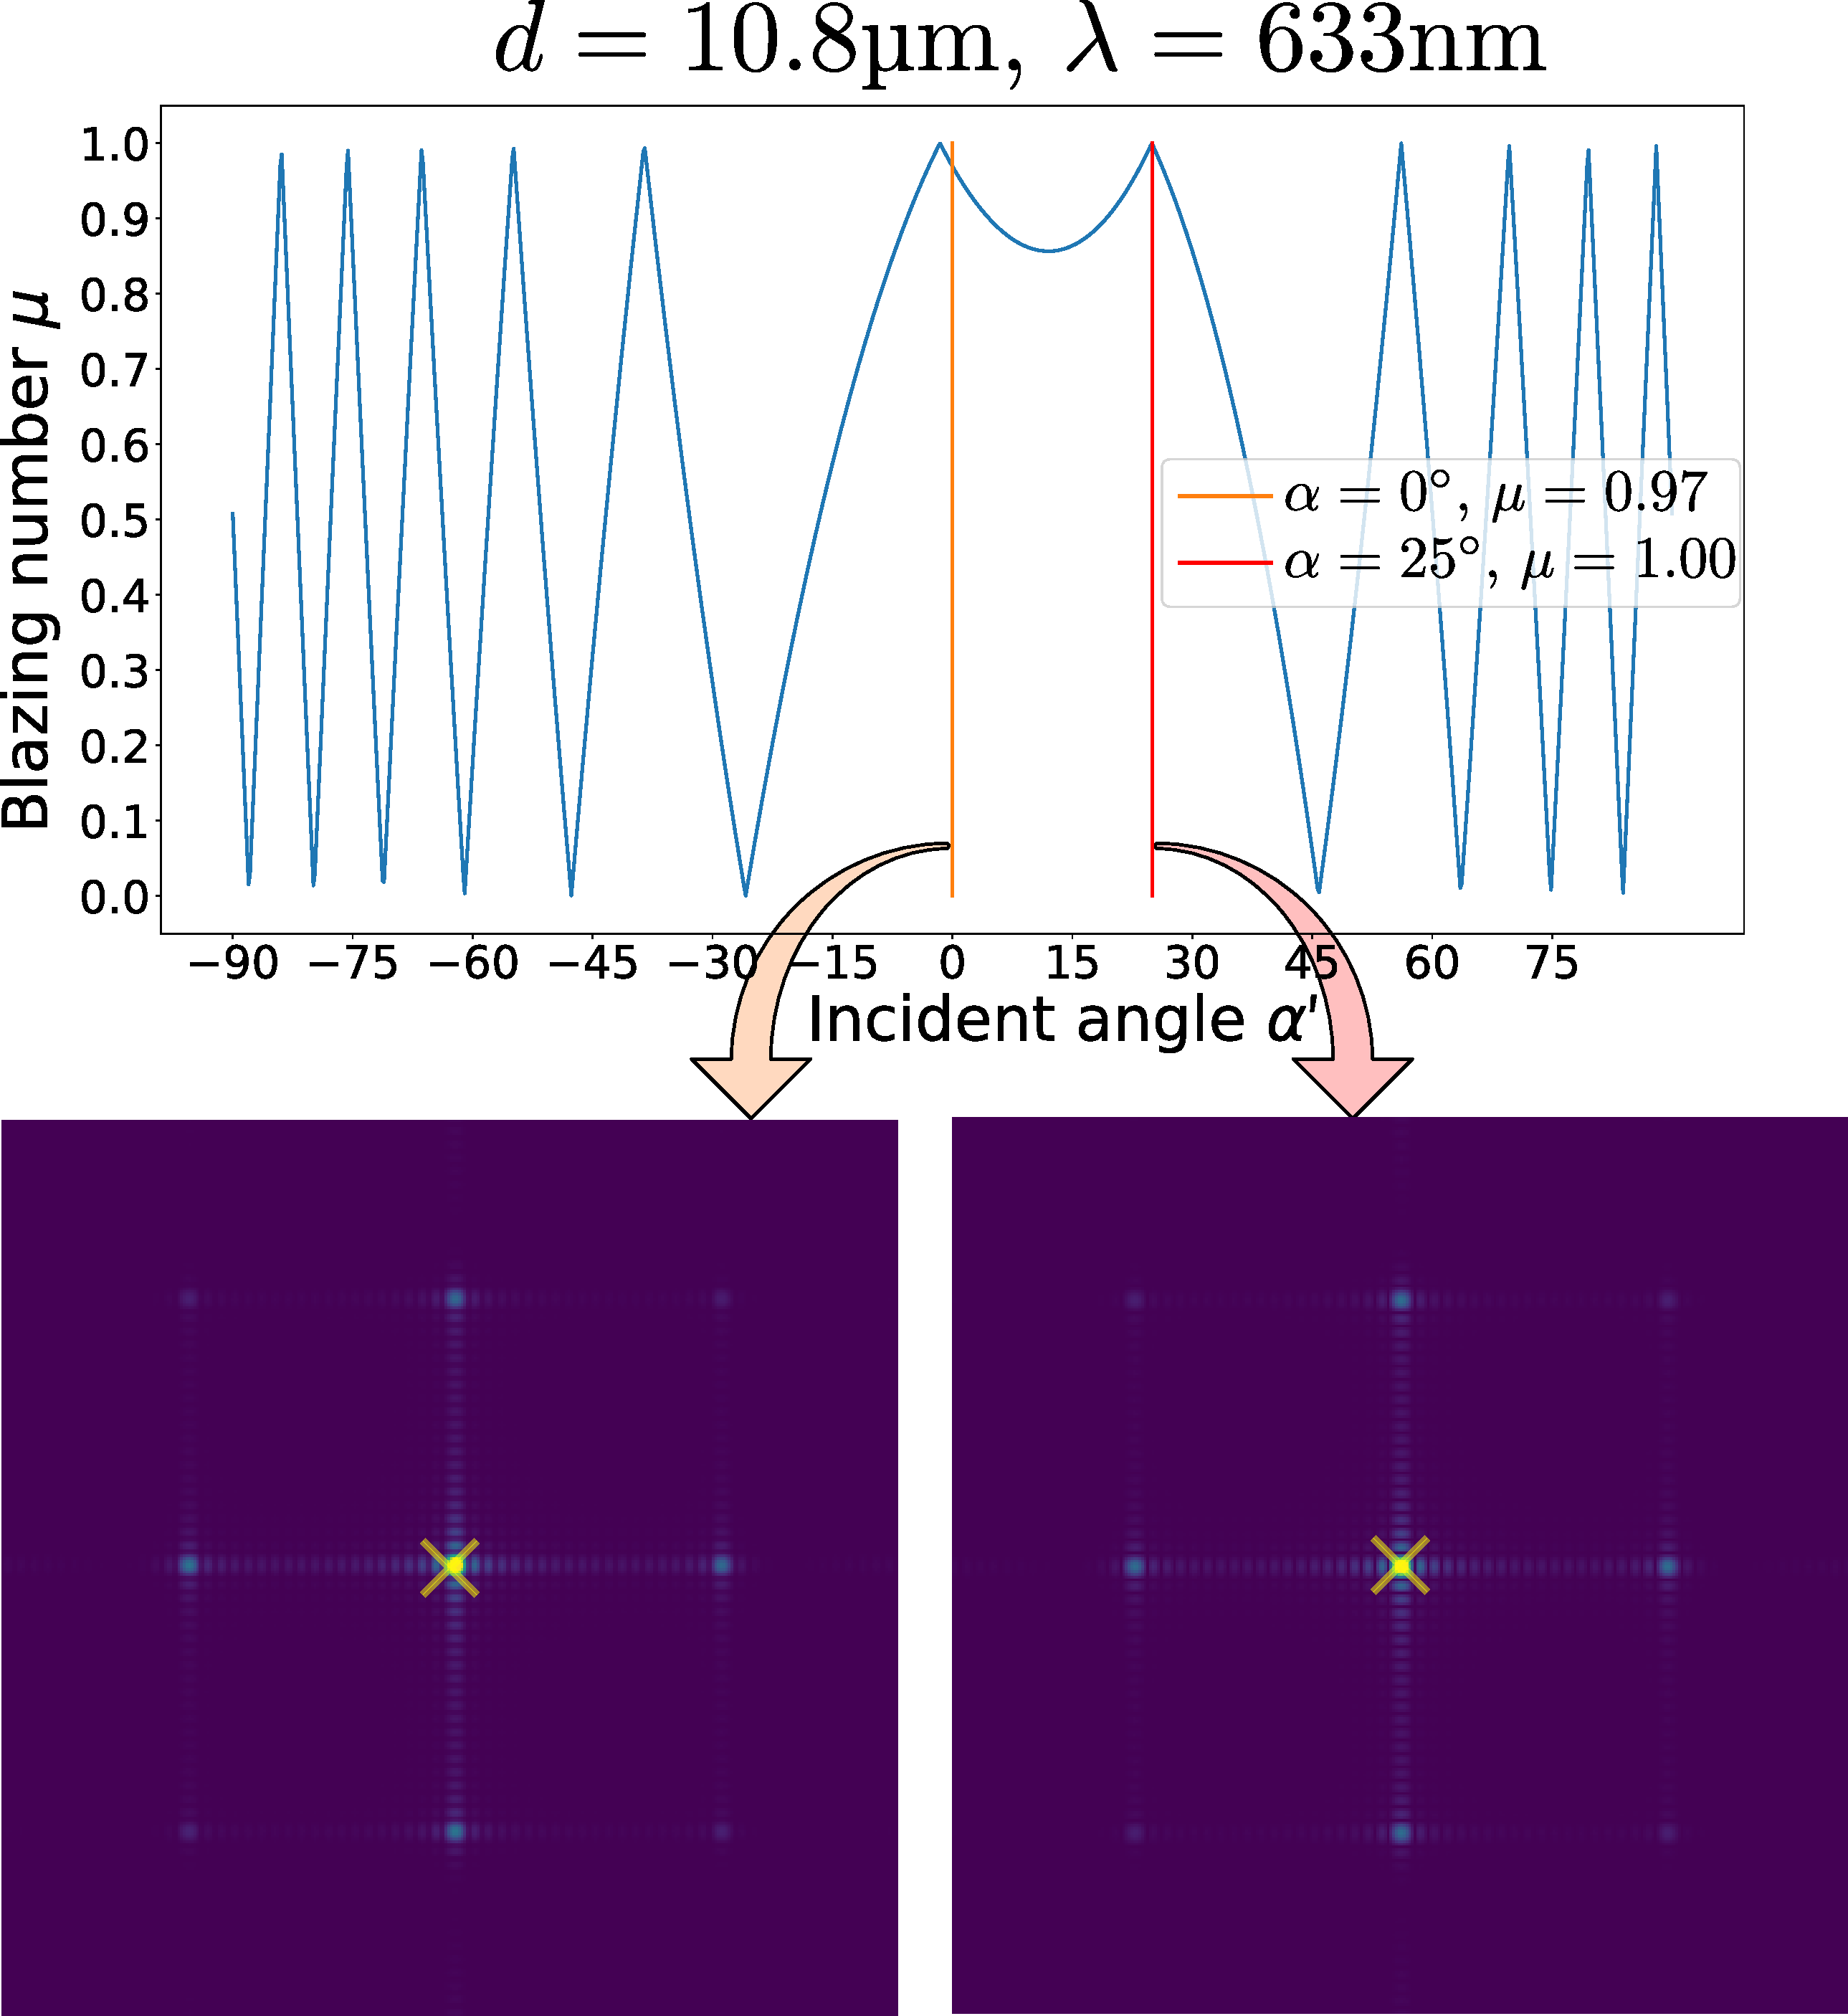
\includegraphics[width = \textwidth]{images/mu_108.pdf}
  \end{subfigure}
  \caption{
  \textbf{Blazed number and far field diffraction pattern for...}
 ...
  }
  \label{fig:mu76}
\end{figure}

\subsection{Modulation cross-talk}

In practice, we place a pinhole or iris to select 
one order of diffraction,
corresponding to the {\em on} state.
Having a small value for the blaze number $\mu$
does not simply limit the amount of light modulated 
due to the reduced diffraction efficiency, 
it also impact the modulation qualoty by introducing cross-talk 
between the two states of the DMD pixels.
For now, we considered that all the pixels are in the same state. 
In a practical use of the DMD,
we need to modulate the state of each pixel individually.
When $\mu$ is close to zero, higher order of diffraction 
still have a non negligible intensity, 
as shown in the 1D case in Fig~\ref{fig:gratings}. 
One consequence is that pixels in the {\em off} state 
may have orders of diffraction that are not blocked by the pinhole, 
and will contribute as a perturbation to the modulated wavefront. 
While this contrinution may seem small, 
it does impact the quality of the modulation 
as the modulation scheme usually requires about half the pixels 
to be in the {\em off}  state for phase modulation~\cite{}, 
and even more for complex modulation schemes~\cite{}.\\

\begin{figure}
  \centering
  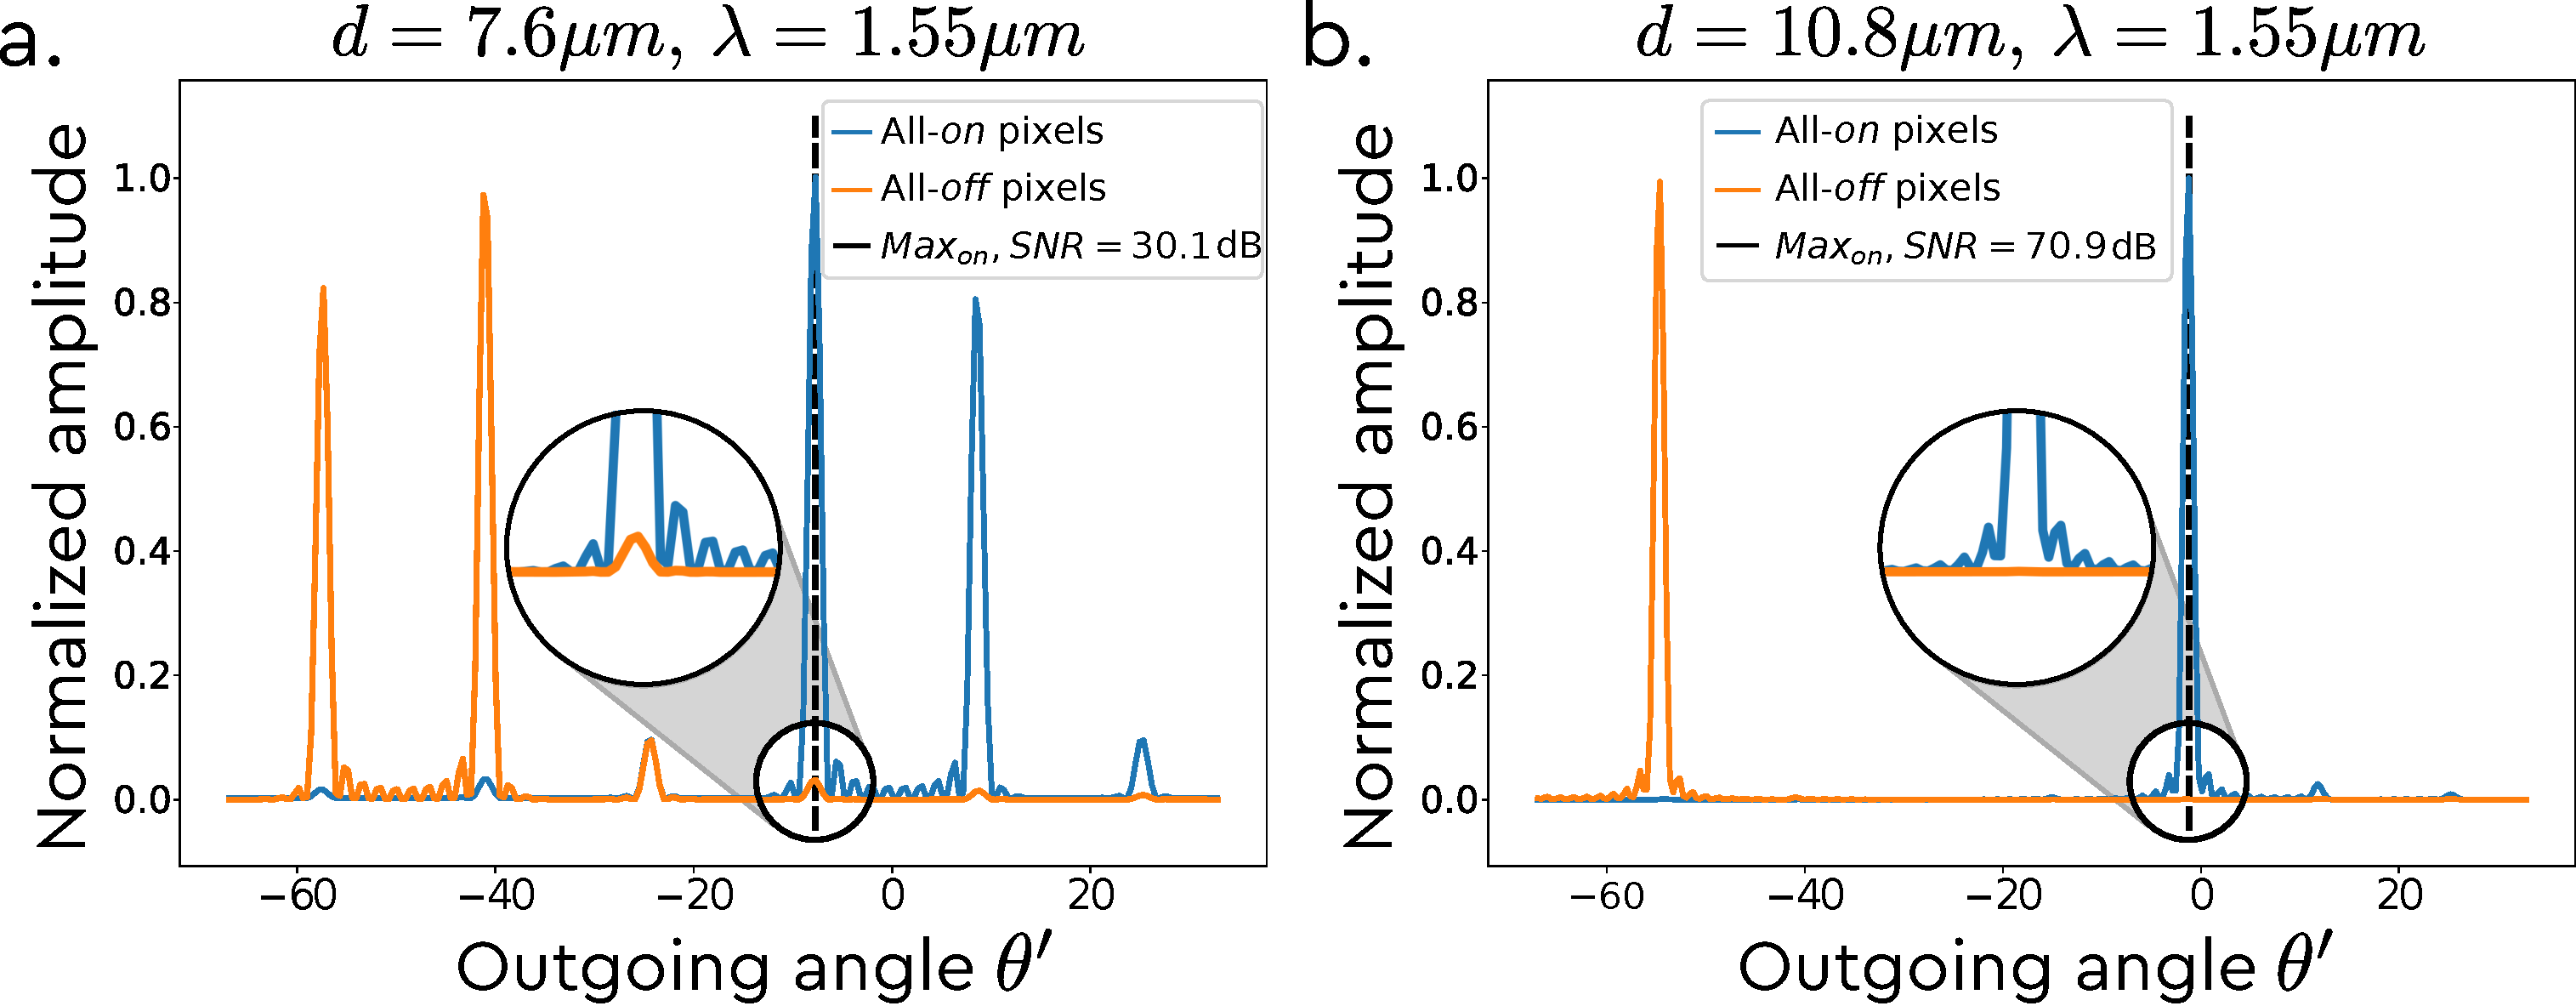
\includegraphics[width = 0.95\textwidth]{images/xtalk.pdf}
  \caption{
  \textbf{Cross-talk between {\em on} and {\em off} states.}
 ...
  }
  \label{fig:xtalk}
\end{figure}
% For an incident angle $\alpha'$ 
% and a reflected angle $\beta'$ 
% in the horizontal plane,
% we can use the grating equation 
% presented in Eq.~\ref{eq:blazed_eq}


\begin{tldr}
  \textbf{TL;DR:}\\
  DMDs act as a blazed grating. 
  For a given operation wavelength,
  we need to find the right pixel pitch 
  to have a good modulation quality 
  and diffraction efficiency.
  \end{tldr}




% Let's consider first a 1D toy model to have a qualitative understanding of the problem.


% Liquid crystal pixels are flat and aligned with the array surface. 
% The periodicity of the pixels makes the device behave as a flat grating. 
% Thus, the reflection angle is the opposite of the incident one compared to the normal of the array plane. 
% That implies that the path coming from each element of the device has the same optical path length 
% (see Fig.~\ref{fig:reflection} left). 


% In a DMD, the modulation is achieved by setting each pixel to one of two states, 
% corrsponding to angles $\pm \theta$ with respect to the the normal of the array plane. 
% It thus acts as a blazed grating.
% Two consecutive pixels, or elements, now give rise to a phase difference 
% between two parallel rays reflected of neighboring pixels (see Fig.~\ref{fig:reflection} right). 
% In the Fourier plane, where we commonly select the zero-th order, all the diffraction orders are shifted compared to the optical axis within the same envelope. In the worst scenario, we can end up with four diffraction orders with approximately the same intensity, each significantly shifted compared to the optical axis. An example is shown in Figure 6. This is almost exactly what I had the first time I set up my DMD while I expected something like in Figure 5.

% Another way of seeing this effect is to consider that the diffraction orders (satisfying the grating equation) do not match anymore the angle of the reflected beam.

% We first use a 1D model to evaluate the effect of the tilt angle on the diffraction pattern. We then use simple numerical calculations to estimate the profile of the diffraction pattern. The full Python code used in this post is available as an IPython Notebook on my GitHub account: blazing_angle_DMD.ipynb.



%%%%%%%%%%%%%%%%%%%%%%%%%%%%%%%%%%%%%%%%%%%%%%%%%%%%%%%%%%%%%%
%%%%%%%%%%%%%%%%%%%%%%%%%%%%%%%%%%%%%%%%%%%%%%%%%%%%%%%%%%%%%%
%%%%%%%%%%%%%%%%%%%%%% ABERRATIONS %%%%%%%%%%%%%%%%%%%%%%%%%%%
%%%%%%%%%%%%%%%%%%%%%%%%%%%%%%%%%%%%%%%%%%%%%%%%%%%%%%%%%%%%%%
%%%%%%%%%%%%%%%%%%%%%%%%%%%%%%%%%%%%%%%%%%%%%%%%%%%%%%%%%%%%%%


\section{Characterizing aberration effects}

\subsection{Presentation of the problem}

While only able to provide a hardware binary amplitude modulation,
DMDs are a powerful tool for wavefront shaping and sensing. 
For these applications, 
aberrations due to the non-flatness of the DMD surface 
are detrimental and need to be characterized and corrected for. 
For LC-SLMs, inhomoegeneities of the surface is usually characterized by the 
manufacturer and the spatial phase profile of the introduced aberrations 
in the plane of the modulator is provided for the working wavelength.
As previously mentioned,
when used for intensity modulation in a plane conjugated to the DMD plane, 
as used in digital projectors, 
the system is not sensitive to aberrations brought by the DMD surface.
For these reasons, this effect is usually not documented, 
and usually not mentioned, in the information provided by the manufacturer 
despite the fact that the deviation from a flat surface
typically reaches few wavelengths~\cite{Brown2021multicolor}.
\\

\subsection{Finding the correction pattern}

In the litterature, different methods have been developped to characterize 
the phase pattern representing the aberrations of the DMD in the 
plane of the modulator. 
Typically, it consists in using a model of the aberations 
and adjusting the parameters to fit the measurements~\cite{Matthes2019Optical,Scholes2019structured, Brown2021multicolor}.
While providing accurate results, 
the implementation of the approach has to be adapted to the specific 
setup condition and may require
additional optical components, 
precise alignments, 
and custom software. 
An other approach consists directly measuring the distorded wavefront, 
either using wavefront sensor, such as a Shack-Hartmann, 
or using interferometry. 
Again, it requires specific hardware and 
a carefully calibrated and stable setup.
In this section, we present a simple method to characterize the aberrations using a lens and a camera. 
This approach can be used for any system prividing a phase modulution, 
such as LC-SLMs or deformable mirrors.\\

\begin{figure}
  \centering
  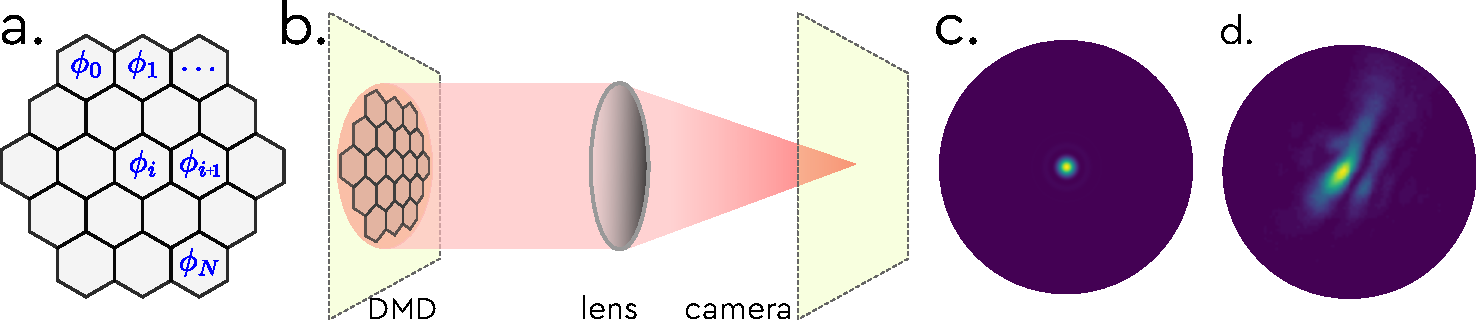
\includegraphics[width = 0.95\textwidth]{images/DMD_abberations_setup.pdf}
  \caption{
  \textbf{Setup for aberration correction.}
 ...
  }
  \label{fig:dmd_aberr_setup}
\end{figure}

He assume that the DMD is configured to provide a phase modulation~\cite{Lee1979binary, RODRIGO}. 
It implies that the modulator can be devided into regions, we call {\em macropixels},
on which the phase can be independently controlled.
We place a lens and a camera in its Fourier plane and illuminate the modulator with a collimated beam 
covering the full desired area of the modualtor we intend to use. 
If there is no or negligible aberrations, the observed intensity pattern 
reseembles the PSF of the lens, i.e. an Airy disk such as presented in Fig.~\ref{fig:dmd_aberr_setup}.c.
However, in partice, we observe a significantly distorted pattern,
such as the one presented in Fig.~\ref{fig:dmd_aberr_setup}.d.\\

We assume the the aberrations introduced by the DMD is smooth and 
can be described by a phase pattern $\phi^\text{aber}$ 
that can be well approximated by a finite number of 
Zernike polynomials $Z_n(r,\theta)$~\cite{Zernike1934beugungstheorie}, such as:

\begin{equation}
  \phi^\text{aber}(r,\theta) \approx \sum_{n=0}^N a_n Z_n(r,\theta) \, .
\end{equation}

The goal is to find and display the phase pattern 
on $\phi_i^\text{corr}$ on each pixel $i$ that best compensate for the aberrations, 
i.e. $\phi_i^\text{corr} = -\phi^\text{aber}(r_i,\theta_i)$.
We create this pattern in the basis of Zernike polynomials

\begin{equation}
  \phi_i^\text{corr} = \sum_{n=0}^N a'_n Z_n(r,\theta) \, ,
\end{equation}

the best correction if obtained for 


\begin{equation}
  a'_n = -a_n \,\, \forall n \in [0..N]\, .
\end{equation}

\begin{figure}
  \centering
  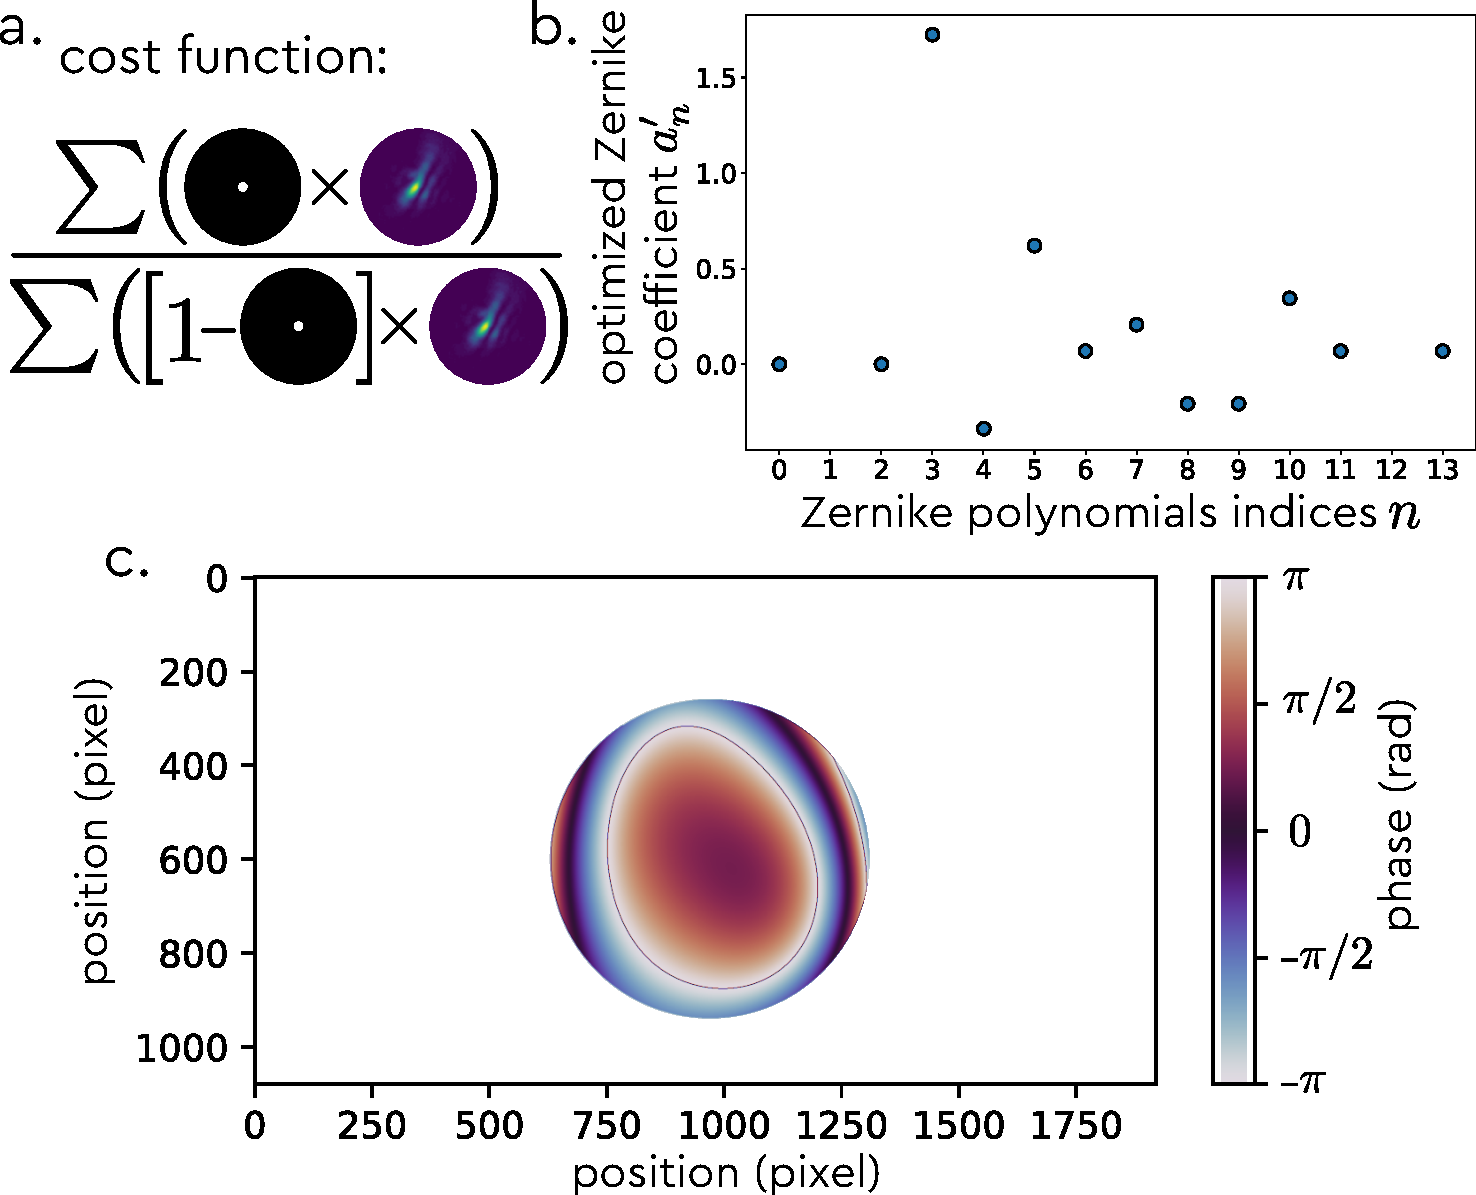
\includegraphics[width = 0.95\textwidth]{images/Zernike_1.pdf}
  \caption{
  \textbf{Correction phase map.}
 ...
  }
  \label{fig:phase_corr}
\end{figure}

We will perform a sequential optimization of the parameters $a_n$ 
to maximize a cost function that is optimial for an ideal correction of the abberations.
To define such a cost function, we first create a mask with a disk 
centered around the maximum of intensity of the initial image (resembling Fig.~\ref{fig:dmd_aberr_setup}.d)
and of radius equivalent to a speckle grain. 
This size does not need to be very very precisely set for the optimization procedure to work, 
and can be found by estimating the size of the ideal PSF, i.e. $r_0 \approx M \frac{\lambda}{2 NA}$, 
with $NA$ the numerical aperture of the optical system and $M$ its magnification.
For a given output image,  we compute the element-wise product between the intensity image measured and the mask and perform a summation.
We start with $a'_n = 0\,\, \forall n \in [0..N]$.
For each parameter, we try different values of $a'_n$,
generate the phases on each pixel so that 
$\phi_i^\text{corr} = \sum_{n=0}^N a'_n Z_n(r_i,\theta_i)$, 
measure the output intensity profile,
and estimate the value the cost function.
We keep for each parameter the value that leads to the highest value.
We repeat the whole process $3$ times for each parameter to 
mitigate the effect of noise or vibration.

\begin{figure}
  \centering
  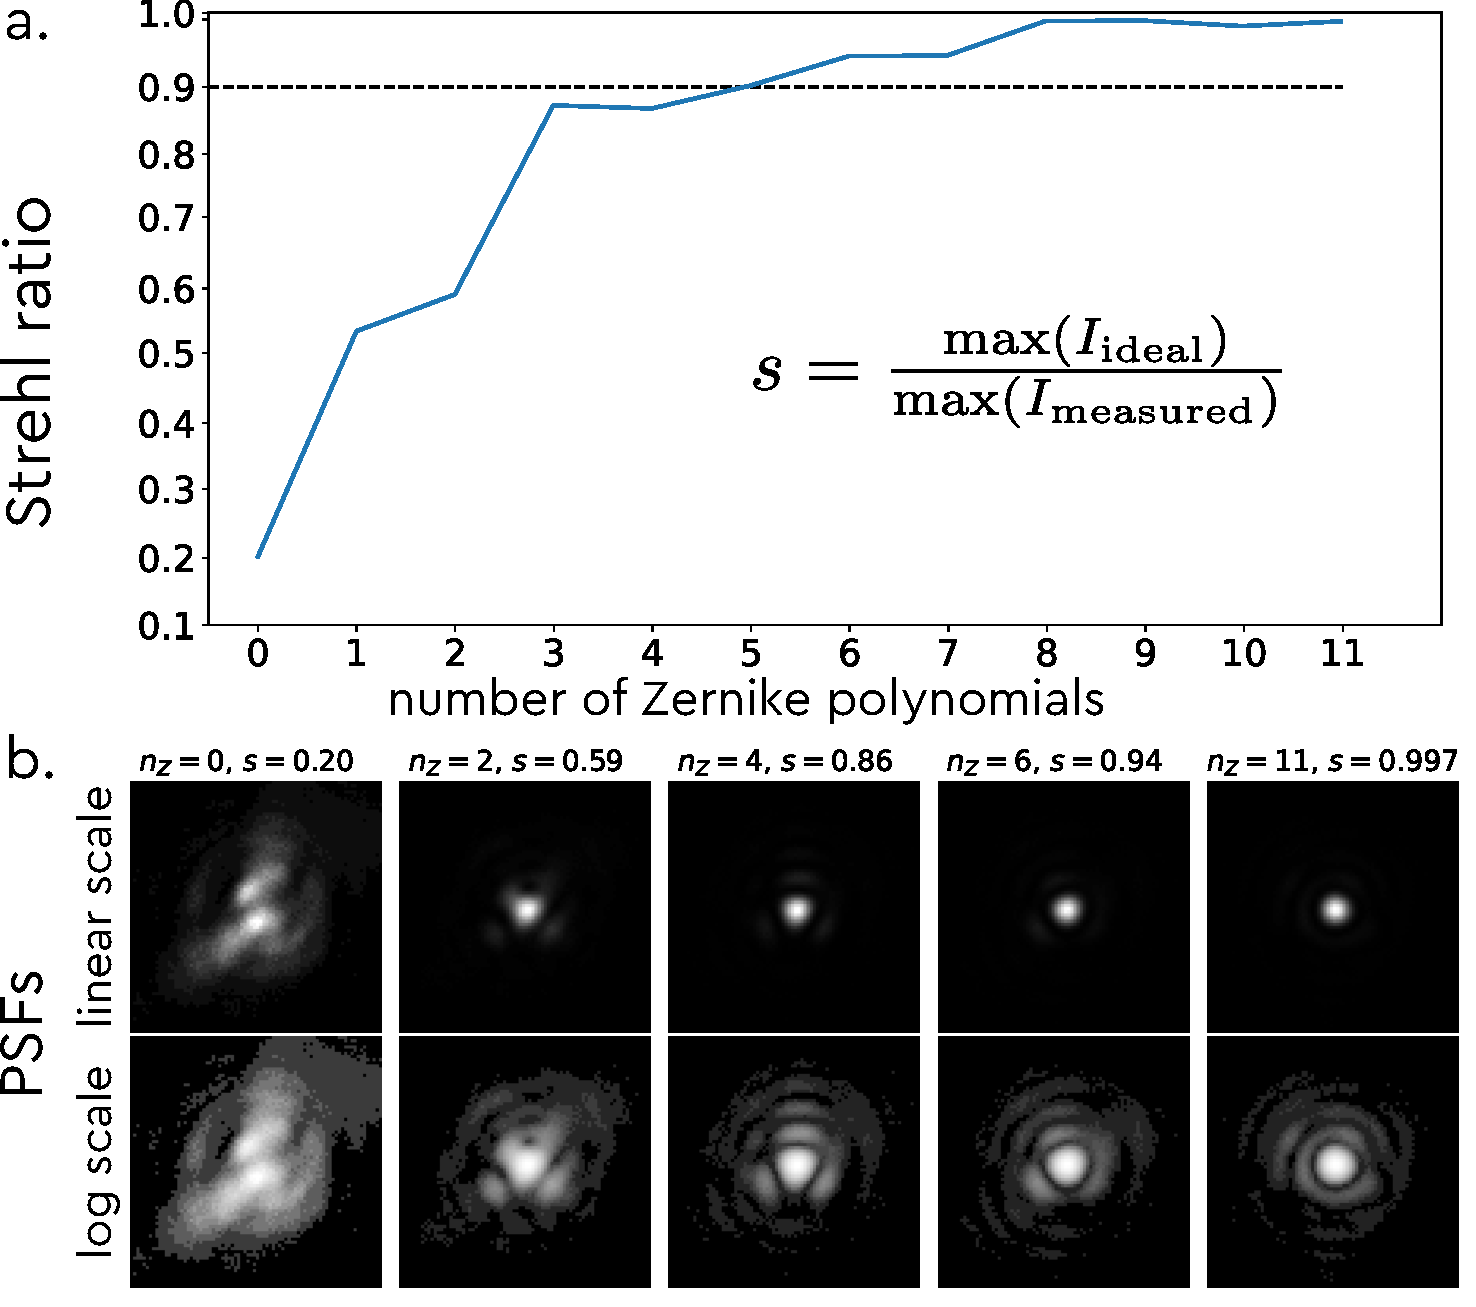
\includegraphics[width = 0.95\textwidth]{images/Zernike_2.pdf}
  \caption{
  \textbf{Effect of Zernike polynomials on the optimizaton of the PSF.}
 ...
  }
  \label{fig:zernike}
\end{figure}


\subsection{Python code example}

We provide in the section Python pieces of code to perform the aberration correction.
We assume that the phase modulation can be controlled using a function 
!display_phase_mask(phase_pattern)! to display a desired phase pattern 
containing real values between $2\pi$.
We remind that phase modulation using a DMD requires an appropirate setup 
and procedure for the generation of the binary pattern that is not detailed here 
but detailed in ths tutorial~\cite{RODRIGO}.
We also assume a function !get_camera_image()! 
that returns the intensity pattern measured by the camera. 
We use the package !aotools!~\cite{Townson2019aotools} for generating Zernike polynomials.

% \lstinputlisting[language=Python, caption=Python example]{code/dmd_aberrations.py}
  

measuring projection of a signal wavefront with a displayed mask and a bucket detector~\cite{}  


\cite{Lee1979binary}


%%%%%%%%%%%%%%%%%%%%%%%%%%%%%%%%%%%%%%%%%%%%%%%%%%%%%%%%%%%%%
%%%%%%%%%%%%%%%%%%%% 4. STABILITY %%%%%%%%%%%%%%%%%%%%%%%%%%%
%%%%%%%%%%%%%%%%%%%%%%%%%%%%%%%%%%%%%%%%%%%%%%%%%%%%%%%%%%%%%

\section{Mechanical and thermal stability}

Unlike the original purpose of the DMD, i.e. ampltiude modulation for video projectors, 
typical scientific applications require a high stability of the generated wavefront. 
This is particularly true for applications in complex media, 
such as strongly scattering media or multimode fiber, 
where a small change in the phase front can lead to a large change in the output intensity profile. 
While LC-SLMs design has been improved and adapted to scientific applicaitons 
over the last decades, 
DMD are still a relatively new tools for wavefront shaping and sensing 
and are prone to instabilities that need to be adressed by the user.
In this section we present the effect of mechanical and thermal instabilities 
and how to limit their impact on the wavefront quality with simple solutions.\\


\subsection{Mechanical stability}

Most DMD kits are composed of two elements, 
the chip itself and the electronics board to control it. 
It can be the standard electronics board for video projectors,
as it is the case for TI evluations kits, 
or a FPGA for fast scientific use, 
as provided by Vialux~\cite{vialux}. 
These electronics come with a fan to cool the chip and the electronics board. 
As the connection between the chip and the electronics board 
used a rigid flat cable, 
the two elements are not mechanically connected.
Vibrations from the board are then transmitted to the chip,
leading to small angle variations of the mirror surface. 
While this effect is without consequences for video projection, 
it can be dramatic applications to complex media 
as their response is highly sensitive to the phase front.\\

Because of this high sensitivy, and since we want to use the DMD 
in the context of complex media, it is simpler to characterize this effect 
directly on the system response rather than 
building a different setup to characterize the wavefront itself.
We show an example of such setup in Fig.~\ref{fig:MMF_ref}. 
We expand an laser beam onto the DMD and sent the input light through a multimode fiber. 
While we typically want phase modulation, 
the setup will need additional elements to achieve this task~\cite{}. 
We here simplify the setup for the sake of clarity. 
The output of the fiber interfere with a reference arm in order to measure 
changes of the field.
We then measure the interference pattern using a camera. \\


\begin{figure}
  \centering
  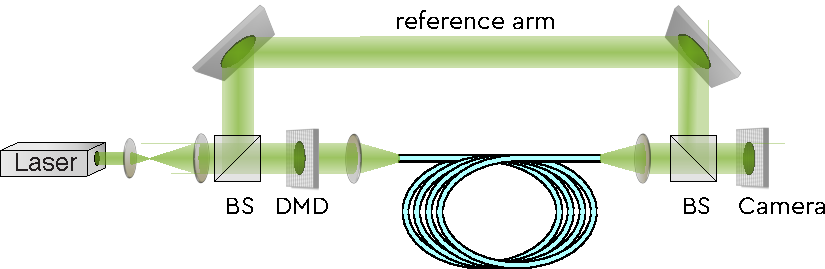
\includegraphics[width = 0.95\textwidth]{images/MMF_ref.pdf}
  \caption{
  \textbf{Measuring stability at the output of a multimode fiber.}
 ...
  }
  \label{fig:MMF_ref}
\end{figure}

We show in the supplementar maeterials~\cite{} an animation of the dynamic pattern. 
We also estimate the phase variation as a function of time. 
In a given region of the image, 
the relation between the phase and the transverse displacement of the fringes
is proportional to the phase, 
with a displacement equal to the fringes period corresponding to $2\pi$.
We show in Fig.~\ref{fig:phase_vibrations} (red curve) 
the fluctuation of the phase over time presenting fast oscillations
due to the mechanical vribration communicated by the board.\\

\begin{figure}
  \centering
  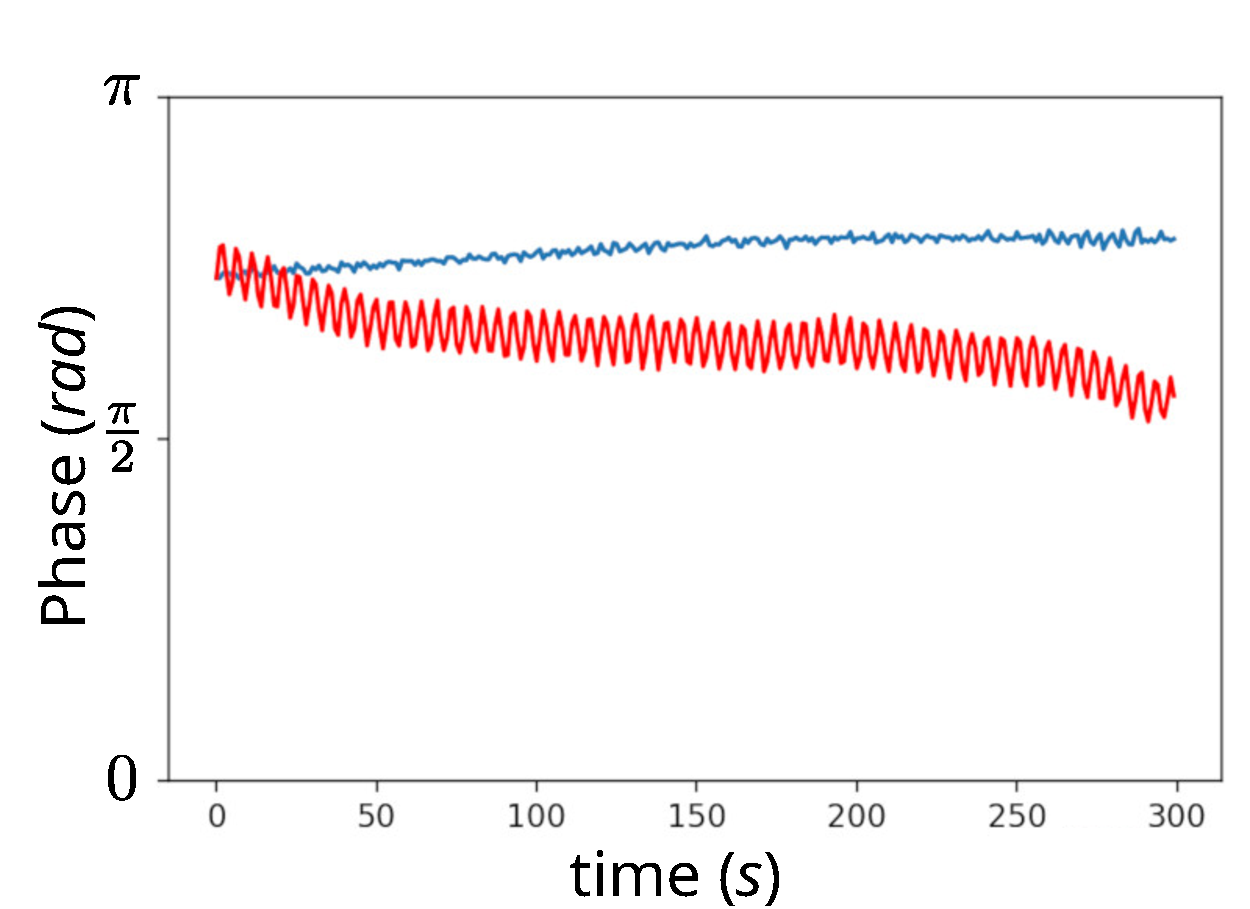
\includegraphics[width = 0.75\textwidth]{images/phase_vibrations.pdf}
  \caption{
  \textbf{Vibration indiced phase fluctuations.}
 ...
  }
  \label{fig:phase_vibrations}
\end{figure}

A simple but efficient solution consists in dumping the vibrations
at the level of the flat cable by clamping the cable with soft maeterial, 
as illustrated in Fig.~\ref{fig:dumping}. 
It can be done with off the shelf material.
We use here simple foam material used for packaging clamped to the cable 
using two metallic plates, screws, and nuts.
We observe a significant reduction of the phase fluctuations 
as shown in Fig.~\ref{fig:phase_vibrations} (blue curve).\\

\begin{figure}
  \centering
  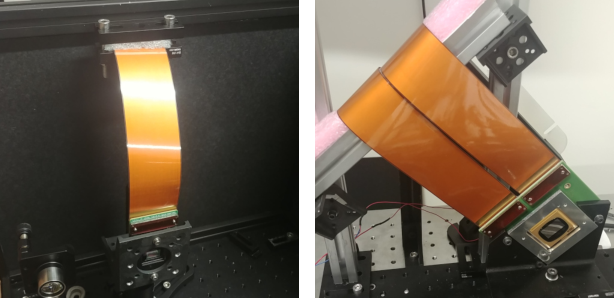
\includegraphics[width = 0.95\textwidth]{images/dumping.pdf}
  \caption{
  \textbf{Dumping mechanical vibrations.}
 ...
  }
  \label{fig:dumping}
\end{figure}

\subsection{Thermal stability}

Electronics used to control the DMD chip heat up during operation.
This effect depends on the frame rate. 
In particular, it is important to notice that this effect is important when 
a sequence is running on the DMD, and is limited when the DMD is powered 
but without any sequence running.
Changes of temperature has the effect of deforming the surface of the chip 
and potentially changing the phase introduced by the glass protecting window.
This has the effect of introducing low order aberrations that degrade the quality of the wavefront.
While this effect is relatively less important than the ones due to 
static aberrations and mechanical instabilities detailed previously, 
it still have a significant impact on the response of a complex medium 
when using a DMD to modulate the input wavefront.\\

The first step consists in characterizing the effect of temperature. 
While a precise effect on the wavefront itself can be measured~\cite{Rudolf2021thermal}, 
it is once again usually more convenient and relevant to measure the effect directly on the response of the system studied.



Thermal stability~\cite{Rudolf2021thermal}

\begin{equation}
C(t) = 
  \frac{
    \left\langle 
     \bar{I}(\vec{r}, t) \bar{I}(\vec{r}, t=0) 
     \right\rangle_{\vec{r}}
  }{
    \sqrt{
     \left\langle 
      \bar{I}(\vec{r}, t)^2 
     \right\rangle_{\vec{r}}
     \left\langle 
      \bar{I}(\vec{r}, t=0)^2 
     \right\rangle_{\vec{r}}
    }
  }
\end{equation}

\begin{figure}[ht]
  \centering
  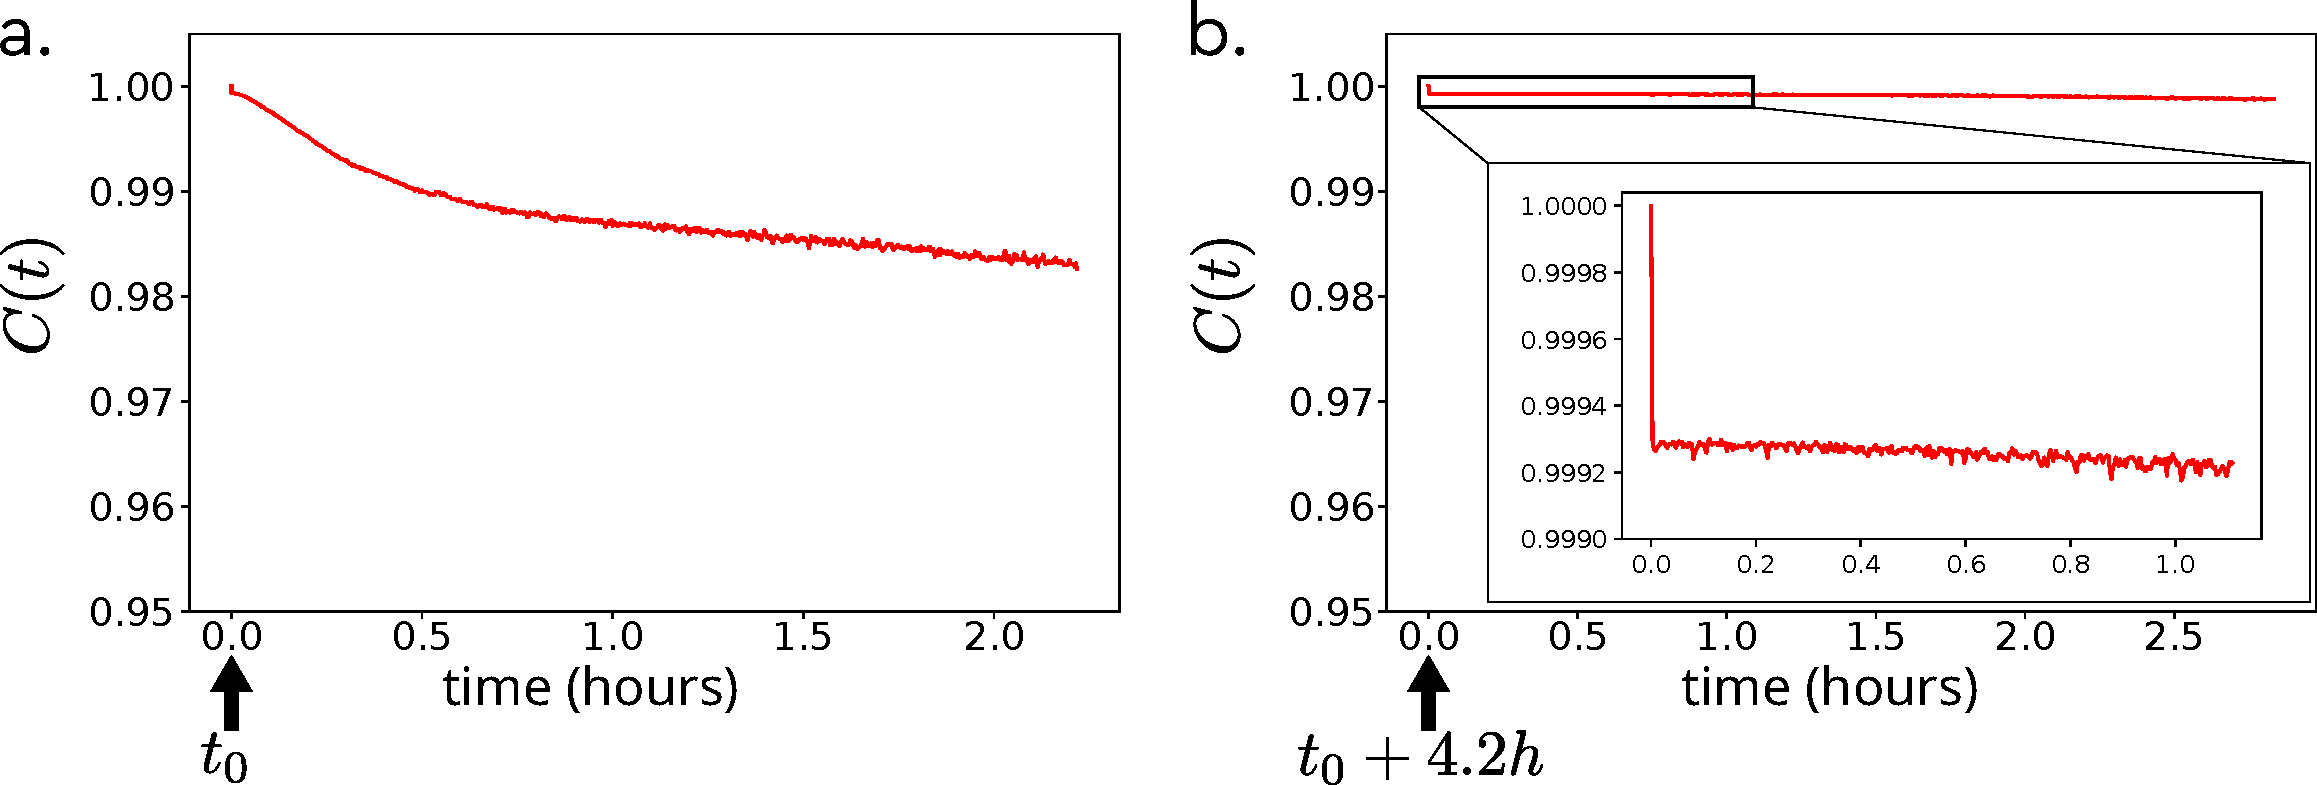
\includegraphics[width = 0.95\textwidth]{images/DMD_decorrelation_T.pdf}
  \caption{
  \textbf{Effect of temperature.}
    ...
  }
  \label{fig:Cizmar_1}
\end{figure}



\begin{figure}
  \centering
  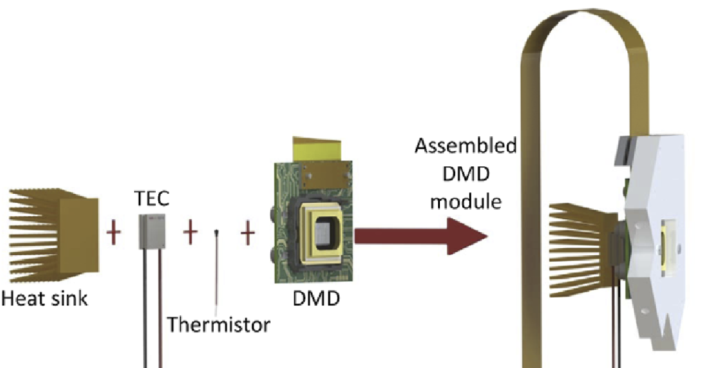
\includegraphics[width = 0.65\textwidth]{images/Cizmar_1.pdf}
  \caption{
  \textbf{Thermal stabilization of the DMD chip.}
    Image adapted from~\cite{Rudolf2021thermal}.
  }
  \label{fig:decorr_T}
\end{figure}

\begin{tldr}
\textbf{TL;DR:}\\
DMDs take about an hour to thermaly stabilize when a sequence is running. 
It can conuntered by using a thermoelectric cooler 
and a temperature sensor. 
It can also be simply mitigated by letting a sequence running for few hours
before starting the experiment. 
\end{tldr}

\section{Control Vialux DMDs with Python}

\cite{hofling2004alp}

\cite{popoff2016alp4lib}

\section{Acknowledgments}
Authors wishing to acknowledge assistance or encouragement from 
colleagues, special work by technical staff or financial support from 
organizations should do so in an unnumbered `Acknowledgments' section 
immediately following the last numbered section of the paper. In \verb"iopart.cls" the 
command \verb"\ack" sets the acknowledgments heading as an unnumbered
section.

\section{Bibliography}


\bibliographystyle{unsrt}
\bibliography{biblio}

\end{document}

